% =================================================================================================
% File:			processi_di_supporto.tex
% Description:	Definisce il capitolo dei processi di supporto
% Created:		2014-12-11
% Author:		Santacatterina Luca
% Email:		santacatterina.luca@mashup-unipd.it
% =================================================================================================
% Modification History:
% Version		Modifier Date		Change											Author
% 0.0.1 		2014-12-11 			Inizializzazione del file						Santacatterina Luca
% =================================================================================================
% 0.0.2 		2015-01-13 			Prima stesura generale							Santacatterina Luca
% =================================================================================================
% 0.0.3			2015-01-20			corretti errori ortografici						Tesser Paolo
% =================================================================================================
% 1.0.1			2015-02-25			aggiornamento tracciamento						Faccin Nicola
% =================================================================================================
% 1.0.2			2015-03-17			aggiunta parte test								Faccin Nicola
% =================================================================================================

% CONTENUTO DEL CAPITOLO

\section{Processi di Supporto}

	\subsection{Processo di documentazione}

		\subsubsection{Attività}

			\paragraph{Documentazione}
			Con il processo di documentazione, il gruppo \groupName{} intende riportare tutte le informazioni acquisite durante il ciclo di vita del software.
			In particolare si andranno ad identificare gli standard per la creazione e stesura dei documenti, nonché tutti i processi atti a rendere i documenti formalmente corretti.


		\subsubsection{Procedure}

			\paragraph{Gestione dei documenti}
			Per ogni documento che il \roleProjectManager{} ritiene utile essere steso dovrà essere generato con appositi tools messi a disposizione. Essi permettono di mantenere un certo ordine e rigore logico.

				\subparagraph{Creazione di un nuovo documento}
				Ogni qualvolta il \roleProjectManager{} voglia creare un nuovo documento dovrà eseguire i seguenti passi:
				\begin{enumerate}
					\item posizionarsi all'interno della cartella \emph{documenti} presente nel repository;
					\item invocare il comando \emph{make nome\textunderscore del\textunderscore documento}.
				\end{enumerate}
				Al termine dell'esecuzione dello script sarà presente una nuova cartella già rinominata correttamente con all'interno presenti tutti i file utili per l'inizio della stesura del nuovo documento.

				\subparagraph{Avanzamento di un documento}
				Alla fine di ogni avanzamento il documento dovrà essere sottoposto a molteplici procedure. Essi possono essere così definite:
				\begin{enumerate}
					\item l'assegnatario dovrà effettuare l'upload del documento all'interno del branch predisposto presente nel repository;
					\item l'assegnatario segnerà come completato il ticket assegnatogli;
					\item il \emph{Verificatore} riceverà automaticamente una mail con la conferma dell'avvenuta conclusione;
					\item il \roleVerifier{} assegnerà un ticket per la risoluzione de problema al redattore del documento;
					\item qualora il documento sia corretto si procederà alla chiusura del ticket, avvisando automaticamente il \roleProjectManager{}, che a sua volta provvederà a contrassegnare il documento come approvato. Altrimenti il \roleVerifier{} assegnerà nuovi ticket al redattore. In seguito il redattore provvederà a eseguire di nuovo tutti i passi del seguente elenco;
				\end{enumerate}

			\paragraph{Gestione del glossario}
			Ogni membro, a seconda di chi il \roleProjectManager{} riterrà opportuno, potrà andare a redigere il glossario. \\
				\subparagraph{Inserimento di un termine}
				In un apposito documento creato su Google Drive, ogni componente che durante la stesura di un documento andrà ad imbattersi in parole che possono risultare ambigue al lettore dovrà inserire quel termine nel documento.

				\subparagraph{Eliminazione di un termine}
				L'incaricato alla stesura del \docNameVersionGlo{} andrà a prendere i termini presenti nel documenti in Google Drive e ad inserirli in ordine alfabetico. Una volta inserito il vocabolo provvederà alla sua rimozione da Google Drive.

				\subparagraph{Inserimento termine nei documenti} % (fold)
				\label{subp:inserimento_termine_nei_documenti}
				Una volta terminata la stesura del \docNameVersionGlo{} l'\roleAdministrator{} provvederà ad eseguire gli script necessari all'inserimento dei termini ambigui seguendo la seguente procedura da terminale:
					\begin{enumerate}
						\item dalla root del repository entrare nella cartella script ed invocare il comando:
							\begin{center}
								\textbf{make glossterm}
							\end{center}
						\item ritornare alla root ed entrare nella cartella documenti. Invocare da li il comando:
							\begin{center}
								\textbf{make gloss}
							\end{center}
					\end{enumerate}
				\noindent
				Una volta terminata l'esecuzione dell'ultimo script i documenti finali saranno stati generati e l'\roleAdministrator{} avrà terminato il suo compito.

				% subparagraph inserimento_termine_nei_documenti (end)


		\subsubsection{Norme}

			\paragraph{Progettazione e sviluppo dei documenti}
			Per ogni documento che si redige si dovrà rispettare un ben preciso layout di sviluppo. Si raccolgono di seguito le informazioni utili per la composizione delle prime pagine, le sezioni e le norme tipografiche da utilizzare in fase di scrittura.

			\paragraph{Versionamento}
			Per ogni documento sviluppato deve essere presente la versione di avanzamento prevista. La classificazione di versionamento deve rispettare le seguenti norme:
			\begin{center}
				X.Y.Z
			\end{center}
			dove:
			\begin{itemize}
				\item \textbf{X}: numero intero che identifica la versione di rilascio ogni qual volta si prepari il documento per una nuova revisione. Ogni incremento di una unità provoca l'azzeramento delle variabili Y e Z;
				\item \textbf{Y}: numero intero che identifica la versione dopo aver passato la fase di verifica. Ogni incremento di una unità provoca l'azzeramento della variabile Z;
				\item \textbf{Z}: numero intero che identifica la versione modificata del documento da parte del redattore. Ogni modifica effettuata provoca l'incremento di una unità.
			\end{itemize}


			\paragraph{Template}
			Al fine di ottenere dei documenti formattati correttamente si è predisposto un template in \LaTeX{} da seguire scrupolosamente. Esso deve essere utilizzato come linea guida per lo sviluppo dei documenti. Ogni tipologia di documento, prima pagina, indici, contenuti interni, lettere hanno uno stile definito in maniera univoca. Esso ne permette una gestione capillare ed omogenea.\\
			Verrà definita inoltre un intestazione per ogni file \emph{.tex} nel modo seguente:
				\begin{verbatim}
					% ==============================================================
					% File:			nome_del_documento.tex
					% Description:	Definisce il capitolo relativo a ...
					% Created:		aaaa-mm-gg
					% Author:		Cognome Nome
					% Email:		cognome.nome@mashup-unipd.it
					% ==============================================================
					% Modification History:
					% Version	Modifier Date	Change							Author
					% 0.0.1 	aaaa-mm-gg 		Descrizione del cambiamento		Cognome Nome

				\end{verbatim}
			\noindent

			\paragraph{Struttura dei documenti}
			Per facilitare la stesura e la gestione si è provvisto alla creazione di un cartella per ogni documento, essa è ha come titolo il nome del documento.\\
			Nella root della cartella è presente il file che gestisce il contenuto della prima pagina. Esso ha il compito di includere tutti gli stili e a linkare tutte le sezioni utili alla costruzione del documento.\\
			All'interno della cartella \emph{content} sono presenti tutti i file, divisi per capitolo, contenti il testo dell'intero documento.\\
			Le cartelle \emph{diagrams} e \emph{images} hanno il compito di contenere i relativi diagrammi ed immagini usati nei singoli documenti.\\
			Nella cartella \emph{doc\textunderscore to\textunderscore modify} sono presenti due file, il primo \emph{content\textunderscore files.tex} raggruppa tutti i sotto capitoli e li ordina in base alle scelte dell'utente. Il secondo file \emph{history.tex} contiene la storia della creazione e modifica apportata al documento.

				\subparagraph{Prima pagina}
				La prima pagina contiene un elenco delle caratteristiche fondamentali del documento quali:
				\begin{itemize}
					\item logo del progetto;
					\item logo, nome ed email del gruppo;
					\item nome del documento;
					\item versione del documento;
					\item data redazione del documento;
					\item cognome e nome dei redattori del documento;
					\item cognome e nome dei verificatori del documento;
					\item cognome e nome dell'approvatore del documento;
					\item lista di distribuzione del documento;
					\item uso interno o esterno del documento;
					\item sommario contenente una breve descrizione del documento.
				\end{itemize}

				\subparagraph{Diario delle revisioni}
				Successivamente nella seconda pagina è presente l'elenco delle revisioni apportate al documento. Esso risulta utile per il tracciamento in fase di elaborazione del documento. Permette di conoscere l'autore delle rispettive sezioni. L'elenco è formato da:
				\begin{itemize}
					\item descrizione della modifica apportata al documento;
					\item cognome, nome e ruolo dell'autore della modifica;
					\item data della modifica;
					\item versione del documento dopo la modifica.
				\end{itemize}

				\subparagraph{Indici}
				Subito dopo il \emph{Diario delle revisioni} è presente l'indice generale del documento. Esso è reperibile in tutti i documenti ad esclusione del \docGlossary.\\
				Nella parte iniziale l'indice fa rifermento ai capitoli e sotto capitoli.\\
				Se presenti immagini e/o tabelle, in automatico è possibile trovare anche il relativo indice associato.

				\subparagraph{Formattazione di una pagina}
				Tutti i documenti descrittivi sono formati da una intestazione è da un piè di pagina ben definito.\\
				Sono presente due bande di colore grigio chiaro agli estremi del documento.\\
				Nella parte alta del documento a sinistra si trova il logo ed il nome del gruppo, mentre nella parte destra il titolo del capitolo principale.\\
				Nella parte inferiore del documento partendo da sinistra è possibile trovare il nome del documento con la relativa versione.\\
				Nella parte destra è presente il numero di pagina formato da ``Pagina X di Y", dove con ``X" si indica la pagina corrente e con ``Y" il numero totale di pagine presenti ad esclusione della prima pagina, del diario delle revisioni e degli indici.

			\paragraph{Suddivisione sezioni documenti}

				\subparagraph{Studio di Fattibilità} Il documento raccoglie le motivazioni e le considerazioni che il gruppo ha elaborato per l'accettazione o meno del progetto da sviluppare. All'interno del documento può essere presente un'analisi che ha portato all'esclusione di altri capitolati.\\
				Il documento è di tipo interno.

				\subparagraph{Norme di Progetto} Il documento raccoglie tutte le attività, norme, procedure e strumenti che il gruppo adotterà durante lo sviluppo del progetto se esso verrà concesso.\\
				Il documento è di tipo interno.

				\subparagraph{Piano di Progetto} Il documento specifica la pianificazione impiegata per lo svolgimento del progetto. Sono contenute tutte le attività con le relative tempistiche e i relativi rischi. Sono inoltre presenti le specifiche di ogni risorsa impiegata;\\
				Il documento è di tipo esterno.

				\subparagraph{Piano di Qualifica} Il documento specifica le strategie applicate al capitolato per ottenere gli obiettivi di qualità. Sono inoltre presenti le attività di verifica e pianificazione con i relativi test che si andranno a sviluppare. \\
				Il documento è di tipo esterno.

				\subparagraph{Analisi dei Requisiti} Il documento identifica e descrive i requisiti necessari all'implementazione del progetto. Saranno inoltre integrati i casi d'uso ed i requisiti utili allo sviluppo del progetto. Saranno altresì presenti i digrammi grafici di interazione tra utenti e sistema.\\
				Il documento è di tipo esterno.

				\subparagraph{Specifica Tecnica} Il documento identifica una prima progettazione ad altro livello del sistema che si andrà a sviluppare. Saranno individuati e dettagliatamente specificati i design pattern utilizzati nel progetto.\\
				Il documento è di tipo esterno.

				\subparagraph{Definizione di Prodotto} Il documento identifica dettagliatamente il prodotto che si va a sviluppare. Tale documento sarà utilizzato dai programmatori per poter sviluppare il software.\\
				Il documento è di tipo esterno.

				\subparagraph{Glossario} Il documento raccoglie tutti i termini usati nella documentazione e ne riporta una definizione più descrittiva.
				Il documento è di tipo esterno.


			\paragraph{Norme tipografiche}
			Tutti i documenti devono rispettare le seguenti norme tipografiche, utili per mantenere i documenti omogenei tra loro.

				\subparagraph{Stili di testo}
				Molti stili di testo sono già stati definiti ed inclusi in appositi file. \LaTeX{} permette così un forte controllo sulla tipografia, restringendone i campi d'applicazione solamente quando necessario.
				\begin{itemize}
					\item \textbf{Colori}: il testo colorato è previsto solamente nei link. Essi sono di colore blu;
					\item \textbf{Corsivo}: il testo corsivo deve essere utilizzato ogni qual volta si voglia dare enfasi ad una determinata parola/frase;
					\item \textbf{Grassetto}: il testo grassetto deve essere utilizzato nella stesura della prefazione degli elenchi non ordinati e ai soli titoli dei capitoli. Può essere utilizzato nel testo ma con moderazione solamente quanto si intende focalizzare un argomento;
					\item \textbf{Maiuscolo}: l'uso del testo maiuscolo è riservato solamente agli acronimi;
					\item \textbf{Sottolineato}: non è previsto l'uso del testo sottolineato.
				\end{itemize}

				\subparagraph{Punteggiatura}
				L'utilizzo della punteggiatura deve essere coerente per tutti i testi scritti in \LaTeX. Si impone così:
				\begin{itemize}
					\item \textbf{Maiuscole}: il primo carattere di testo maiuscolo è consentito solamente dopo il punto, punto di domanda, punto esclamativo o nell'intestazione di ogni elenco;
					\item \textbf{Numeri}: i numeri dovranno rispettare lo standard SI/ISO 31-0
					\item \textbf{Parentesi}: nel testo è ammesso solamente l'uso di parentesi tonde. Il testo racchiuso tra parentesi non deve mai iniziare o finire con alcun carattere di spaziatura;
					\item \textbf{Punteggiatura}: prima di ogni simbolo di punteggiatura \emph{non deve} essere presente alcun carattere di spaziatura. L'uso del punto servirà solamente per terminare una discussione;
					\item \textbf{Spazi}: non dovranno mai essere presenti spazi doppi, o spazi per la tabulazione.
				\end{itemize}

				\subparagraph{Composizione del testo}
				\begin{itemize}
					\item \textbf{Elenchi non numerati}: ogni singolo elemento deve iniziare con un testo scritto in grassetto e con la prima lettera maiuscola. Ogni singolo punto dell'elenco deve terminare con il punto e virgola. Solamente alla fine è obbligo l'uso del punto;
					\item \textbf{Elenchi numerati}: ogni singolo elemento deve iniziare con il testo scritto in minuscolo. Ogni singolo punto dell'elenco deve terminare con il punto e virgola. Solamente alla fine è obbligo l'uso del punto;
					\item \textbf{Note a piè di pagina}: ogni singola nota a piè di pagina deve iniziare con lettera maiuscola. Tutte le note a piè di pagina devono terminare obbligatoriamente con il punto e virgola;
					\item \textbf{Pedice ``G''}: per tutti gli acronimi e/o termini particolari presenti nei documenti e riportati nel \docGlossary, deve essere presente la notazione tramite pedice ``G''.
				\end{itemize}

				\subparagraph{Formati ricorrenti}
				\begin{itemize}
					\item \textbf{Nomi propri:} tutti nomi propri devono essere espressi nella forma ``Cognome Nome";
					\item \textbf{Date:} ogni data deve essere scritta come indicato dallo standard ISO 8601:\\
						\begin{displaymath}
							AAAA-MM-GG
						\end{displaymath}
						dove:
						\begin{itemize}
							\item \textbf{AAAA}: rappresenta l'anno scritto in numero ed in modalità estesa con tutti e quattro i caratteri;
							\item \textbf{MM}: rappresenta il mese scritto in numero ed in modalità estesa con tutti e due i caratteri;
							\item \textbf{GG}: rappresenta il giorno scritto in numero ed in modalità estesa con tutti e due i caratteri.
						\end{itemize}
					\item \textbf{Riferimenti ai documenti}: ogni riferimento ai documenti deve presentare il nome del documento e la sua attuale revisione;
				\end{itemize}

			\paragraph{Componenti grafiche}

				\subparagraph{Immagini}
				Ogni immagine inclusa nei documenti deve essere in formato PDF, meglio se in formato vettoriale in quanto riduce lo spazio occupato e migliora la scalabilità.\\
				Ogni immagine deve essere salvata nell'apposita directory \emph{images} messa a disposizione.\\
				Assieme all'immagine deve essere fornita una descrizione ed una parola chiave per poter riportare nel testo la figura di rifermento.\\
				Il numero viene assegnato automaticamente dal software \LaTeX.

				\subparagraph{Diagrammi}
				Ogni diagramma riportato nei documenti deve essere in formato PDF, meglio se in formato vettoriale in quanto riduce lo spazio occupato e migliora la scalabilità.\\
				Ogni diagramma deve essere salvato nell'apposita directory \emph{diagrams} messa a disposizione.\\
				Assieme al digramma deve essere fornita una descrizione ed una parola chiave per poter riportare nel testo il diagramma di rifermento.\\
				Il numero viene assegnato automaticamente dal software \LaTeX.

				%\subparagraph{Tabelle}

		\subsubsection{Strumenti} % (fold)
		\label{ssub:strumenti}
		Per semplificare ed automatizzare il lavoro sono stati creati alcuni script che verranno lanciati o automaticamente durante una determinata azione sul repository o in maniera manuale dai membri del team quando necessario.
			\paragraph{Script} % (fold)
			\label{par:script_doc}
				\begin{itemize}
					\item \textbf{Generazione struttura documento}: il makefile predisposto per la nuova generazione dei documenti ha il ruolo di effettuare una copia del template di documento ed assegnargli il nome;
					\item \textbf{Compilazione documento}: per la compilazione dei documenti è stato sviluppato un makefile che procede alla compilazione completa del file \LaTeX{} e ne verifica tramite il software GNU Aspell la correttezza ortografica.\\
					Alla fine della compilazione elimina tutti i file temporanei e procede all'apertura del file pdf;
					\item \textbf{Inserimento notazioni termini di glossario}: lo script provvede alla duplicazione della cartella relativa ai documenti e analizza documento per documento, inserendo la notazione  ``G'' in pedice per tutti i termini presenti nel glossario. \\
					Alla fine si crea automaticamente una nuova cartella contenente tutti i documenti compilati;
					\item \textbf{Calcolo indice di Gulpease}: tramite lo script di parsing automatico avviato sul documento è possibile ottenere l'indice di Gulpease all'interno di un file di testo separato;
					\item \textbf{Controllo ortografico}: sul makefile per la compilazione dei file \LaTeX{} è presente l'integrazione del software GNU Aspell per il controllo ortografico che blocca la compilazione e lancia una eccezione specificando il termine da modificare.
				\end{itemize}
			% paragraph script (end)

		% subsubsection strumenti (end)


	\subsection{Processo di verifica}
	Con il processo di verifica si vuole introdurre una approfondita analisi del rispetto dei requisiti fissati prima dell'inizio del progetto.\\
	Tale tecnica permette di aumentare il fattore efficienza/efficacia e di ridurre il tempo impiegato nell'analisi.\\
	Il processo prevede una prima fase di pianificazione e successivamente di verifica.

		\subsubsection{Attività}

			\paragraph{Analisi statica} % (fold)
			\label{par:analisi_statica}
			L'attività di analisi statica è una ben precisa tecnica di verifica, applicabile sia a documenti sia a codice sorgente. Essa viene applicata durante tutto il ciclo di sviluppo del progetto. Ha come obiettivo la ricerca delle anomalie. Un volta individuate possono essere così applicate:
			\begin{itemize}
				\item \textbf{Walkthrough}: il seguente metodo, ricerca all'interno del testo e del codice, tutte le possibili anomalie. L'analisi si basa sulla lettura di tutto il testo.\\
				Dopo aver trovato le varie anomalie si portano in discussione con il redattore del documento e si cerca una risoluzione ottimale. \\
				Tale tecnica può essere usata all'inizio del progetto, in quanto non si ha una visione generale del documento/codice che si sta sviluppando. Permette così ai verificatori di preparare una \emph{checklist}.\\
				Come descritto inizialmente, tale tecnica risulta la più adeguata. Solamente dopo aver stilato una \emph{lista di controllo}, si potrà passare ad una analisi più specifica, usando l'attività di analisi di tipo \emph{inspection};
				\item \textbf{Inspection}: il seguente metodo si basa sulla lettura mirata del documento/codice per analizzarne i difetti. Sarà così possibile usare la lista di controllo per verificare la presenza di errori. Con l'acquisizione di nuove capacità si potrà così ampliare la lista di controllo in modo tale da rendere l'operazione più efficiente/efficace.
			\end{itemize}
			% paragraph analisi_statica (end)

			\paragraph{Analisi dinamica} % (fold)
			\label{par:analisi_dinamica}
			L'attività di analisi dinamica si può applicare solamente a livello software. Può essere applicata all'interno software o per semplicità anche ad una singola porzione di esso.\\
			L'attività prevede l'esecuzioni di test automatici programmati precedentemente, essi servono a verificarne il corretto funzionamento. Essendo uno strumento automatico di verifica, in caso di anomalie il sistema invierà delle notifiche per identificare chiaramente il problema.\\
			Tutti i test applicati si intendono ripetibili, ovvero devono poter essere applicati in qualsiasi momento e ripetuti per tutta la durata del software.\\
			Ogni test deve avere delle caratteristiche ben precise da rispettare, ovvero:
			\begin{itemize}
				\item \textbf{Ambiente}: deve essere riportato necessariamente l'ambiente sia software sia hardware in cui il sistema dovrà eseguire il test. Deve necessariamente essere specificato lo stato iniziale del sistema;
				\item \textbf{Specifica}: devono essere riportati necessariamente i dati in input ed output. Questi serviranno per poter effettuare un test di congruenza;
				\item \textbf{Procedure}: possono essere specificati ulteriori istruzioni per l'esecuzione dei test. Inoltre possono essere riportate istruzioni sulla corretta lettura dei risultati.
			\end{itemize}
			% paragraph analisi_dinamica (end)

			\paragraph{Gestione anomalie}
			Il \roleVerifier, durante le attività di controllo, nel caso si riscontrassero anomalie o discordanze normative avrà il compito di notificarle all'assegnatario del task sul quale sta effettuando la verifica.\\
			Nella sezione \ref{par:Procedure_assegnazione_delle_anomalie}. è indicata la procedura per l'apertura di una nuova anomalia.

			\paragraph{Test} % (fold)
			\label{par:test}
				\subparagraph{Test di unità}
				I test di unità verificano che ogni unità software funzioni a dovere. Attraverso questo si può verificare la correttezza di tutti i moduli base che andranno a comporre il software, limitando così gli errori di implementazione. Questo tipo di test vengono identificati con la sintassi seguente:\\
				 \begin{center}
				 	TU[Codice test]
				 \end{center}

				 \subparagraph{Test di integrazione}
				 I test di integrazione verificano che i moduli verificati singolarmente funzionino anche se integrati tra di loro. Questo aiuta anche a scoprire eventuali problemi non sottolineati nei test precedenti. L'integrazione in oltre non viene fatta solo con moduli interni ma anche con componenti esterne quali librerie e framework.\\
				 Potranno inoltre essere utilizzate delle componenti create ad hoc che simulano i risultati dei moduli non ancora pronti, questo per poter analizzare il risultato di determinati test. Questo tipo di test vengono identificati con la sintassi seguente:\\
				 \begin{center}
				 	TI[Identificativo del componente]
				 \end{center}

				 \subparagraph{Test di sistema}
				 I test di sistema consistono nella validazione del prodotti software. Questi saranno eseguiti solamente quando si ritiene che il prodotto è giunto ad una versione stabile. Si verifica dunque che il prodotto soddisfi tutti i requisiti. Questo tipo di test vengono identificati con la sintassi seguente: \\
				\begin{center}
				 	TS[Tipo requisito][Codice requisito]
				 \end{center}

				 \subparagraph{Test di regressione}
				 I test di regressione vengono eseguiti dopo che un componente è stato modificato. Si eseguono tutti i test fatti precedentemente per verificare che le modifiche fatte non causino problemi agli altri moduli. Grazie al tracciamento si possono ricavare dei test critici, ossia coloro che sono più a rischio in caso di modifica, e quindi da ripetere ogni volta.
				 \subparagraph{Test di validazione}
				 I test di validazione coincidono con il collaudo del prodotto con il proponente. Se tale test è positivo allora significa che il prodotto proposto è abbastanza maturo per essere rilasciato. Questo tipo di test vengono identificati con la seguente sintassi:\\
				 \begin{center}
				 	TV[Tipo requisito][Codice requisito]
				 \end{center}

			\paragraph{Tracciamento} % (fold)
			\label{par:tracciamento}
			L'attività di tracciamento, eseguita dai \emph{Verificatori}, prevede il controllo della corrispondenza dei requisiti definiti nelle fasi precedenti. In oltre ogni requisito deve essere tracciato al componente che lo soddisfa, in modo da garantire che ogni requisito venga soddisfatto. Questo consente anche di misurare il progresso nell'attività di progettazione.
			% paragraph tracciamento (end)


		\subsubsection{Procedure}
		\label{ssub:procedure}

			\paragraph{Procedure d'assegnazione delle anomalie}
			\label{par:Procedure_assegnazione_delle_anomalie}
			L'assegnazione delle anomalie riscontrate da parte del \roleVerifier{} deve avvenire tramite l'uso della piattaforma Asana.\\
			Esistono due tipi di sezioni sulle quali effettuare la segnalazione:
			\begin{itemize}
				\item \textbf{Bug Tracking Document}: sezione dedicata alle anomalie riguardante la documentazione;
				\item \textbf{Bug Tracking Source}: sezione dedicata alle anomalie riguardante il codice sorgente del software.
			\end{itemize}
			\noindent
			\`E necessario fare uso di uno dei due template messi a disposizione, presenti all'interno delle viste sopraelencate.\\
			Per l'assegnazione si devono eseguire i seguenti punti, maggiormente schematizzati nella figura \ref{fig:procedura_assegnazione_anomalie}:
			\begin{enumerate}
				\item definizione del nuovo titolo, contenente nella parte iniziale la dicitura {[}bug{]};
				\item descrizione esplicativa dell'errore riscontrato e punto del riscontro;
				\item assegnazione al membro del gruppo che ha commesso l'errore;
				\item inserimento data di scadenza per la correzione dell'anomalia;
				\item assegnazione del tipo di priorità in base alle norme presenti nella sezione \ref{par:priorita_risoluzione_anomalie}.
			\end{enumerate}
			\noindent
			Il sistema automaticamente provvederà alla notifica del nuovo task attraverso l'invio di una mail.
			\begin{figure}[htbp]
				\centering
				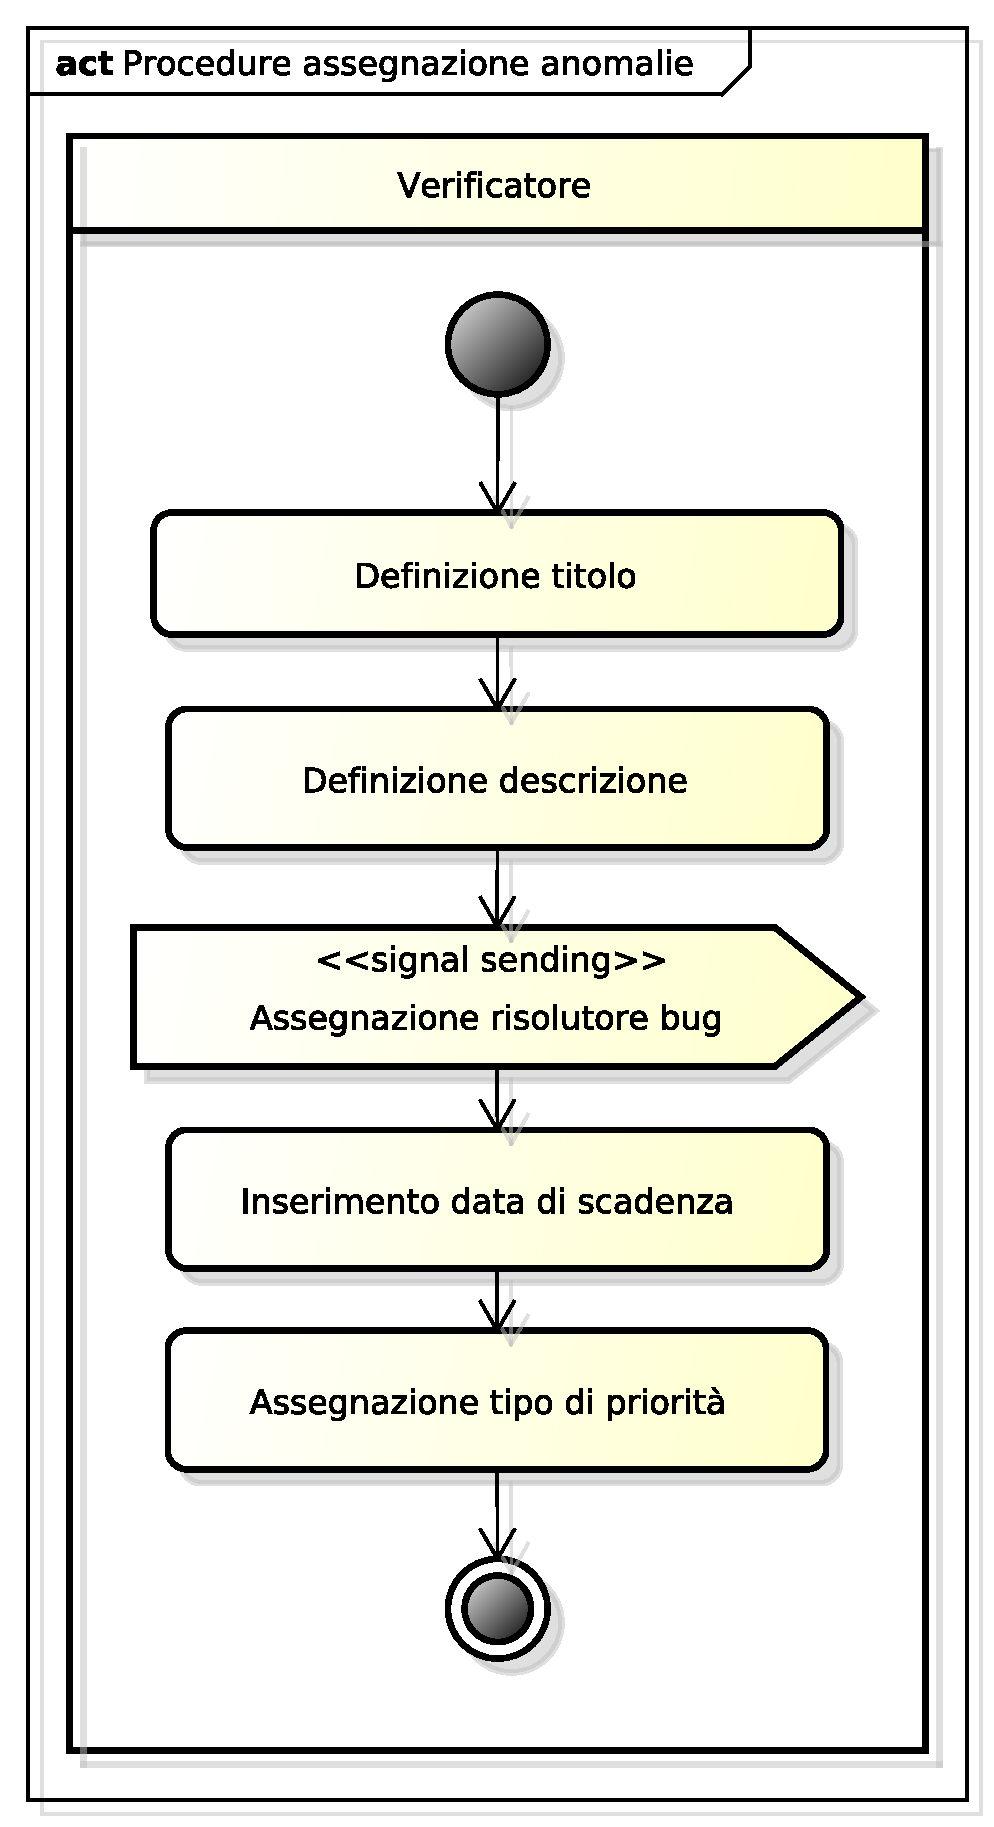
\includegraphics[scale=0.5]{images/proc_assegnazione_anomalie.pdf}
				\caption{Diagramma di attività - procedura assegnazione anomalie}
				\label{fig:procedura_assegnazione_anomalie}
			\end{figure}


			\paragraph{Configurazione sistema di Continuous Integration} % (fold)
			\label{par:configurazione_sistema_di_continuos_integration}
			Ogni membro del gruppo dovrà seguire la seguente procedura per interfacciarsi con il sistema adottato di Continuous Integration \ref{par:wercker} configurato dall'\roleAdministrator.
				\begin{itemize}
					\item accedere al sito \url{http://wercker.com/} tramite l'account di GitHub;
					\item dal menù in alto selezionare la voce ``Create'' e scegliere ``Application'';
					\item selezionare GitHub come provider di Git;
					\item selezionare il repository che interessa (src\_BDSM\_App\_client e src\_BDSM\_App\_server);
					\item premere il pulsante ``Join App'';
					\item ripetere la procedura per entrambi i repository citati al punto 4.
				\end{itemize}

				\begin{figure}[htbp]
					\centering
					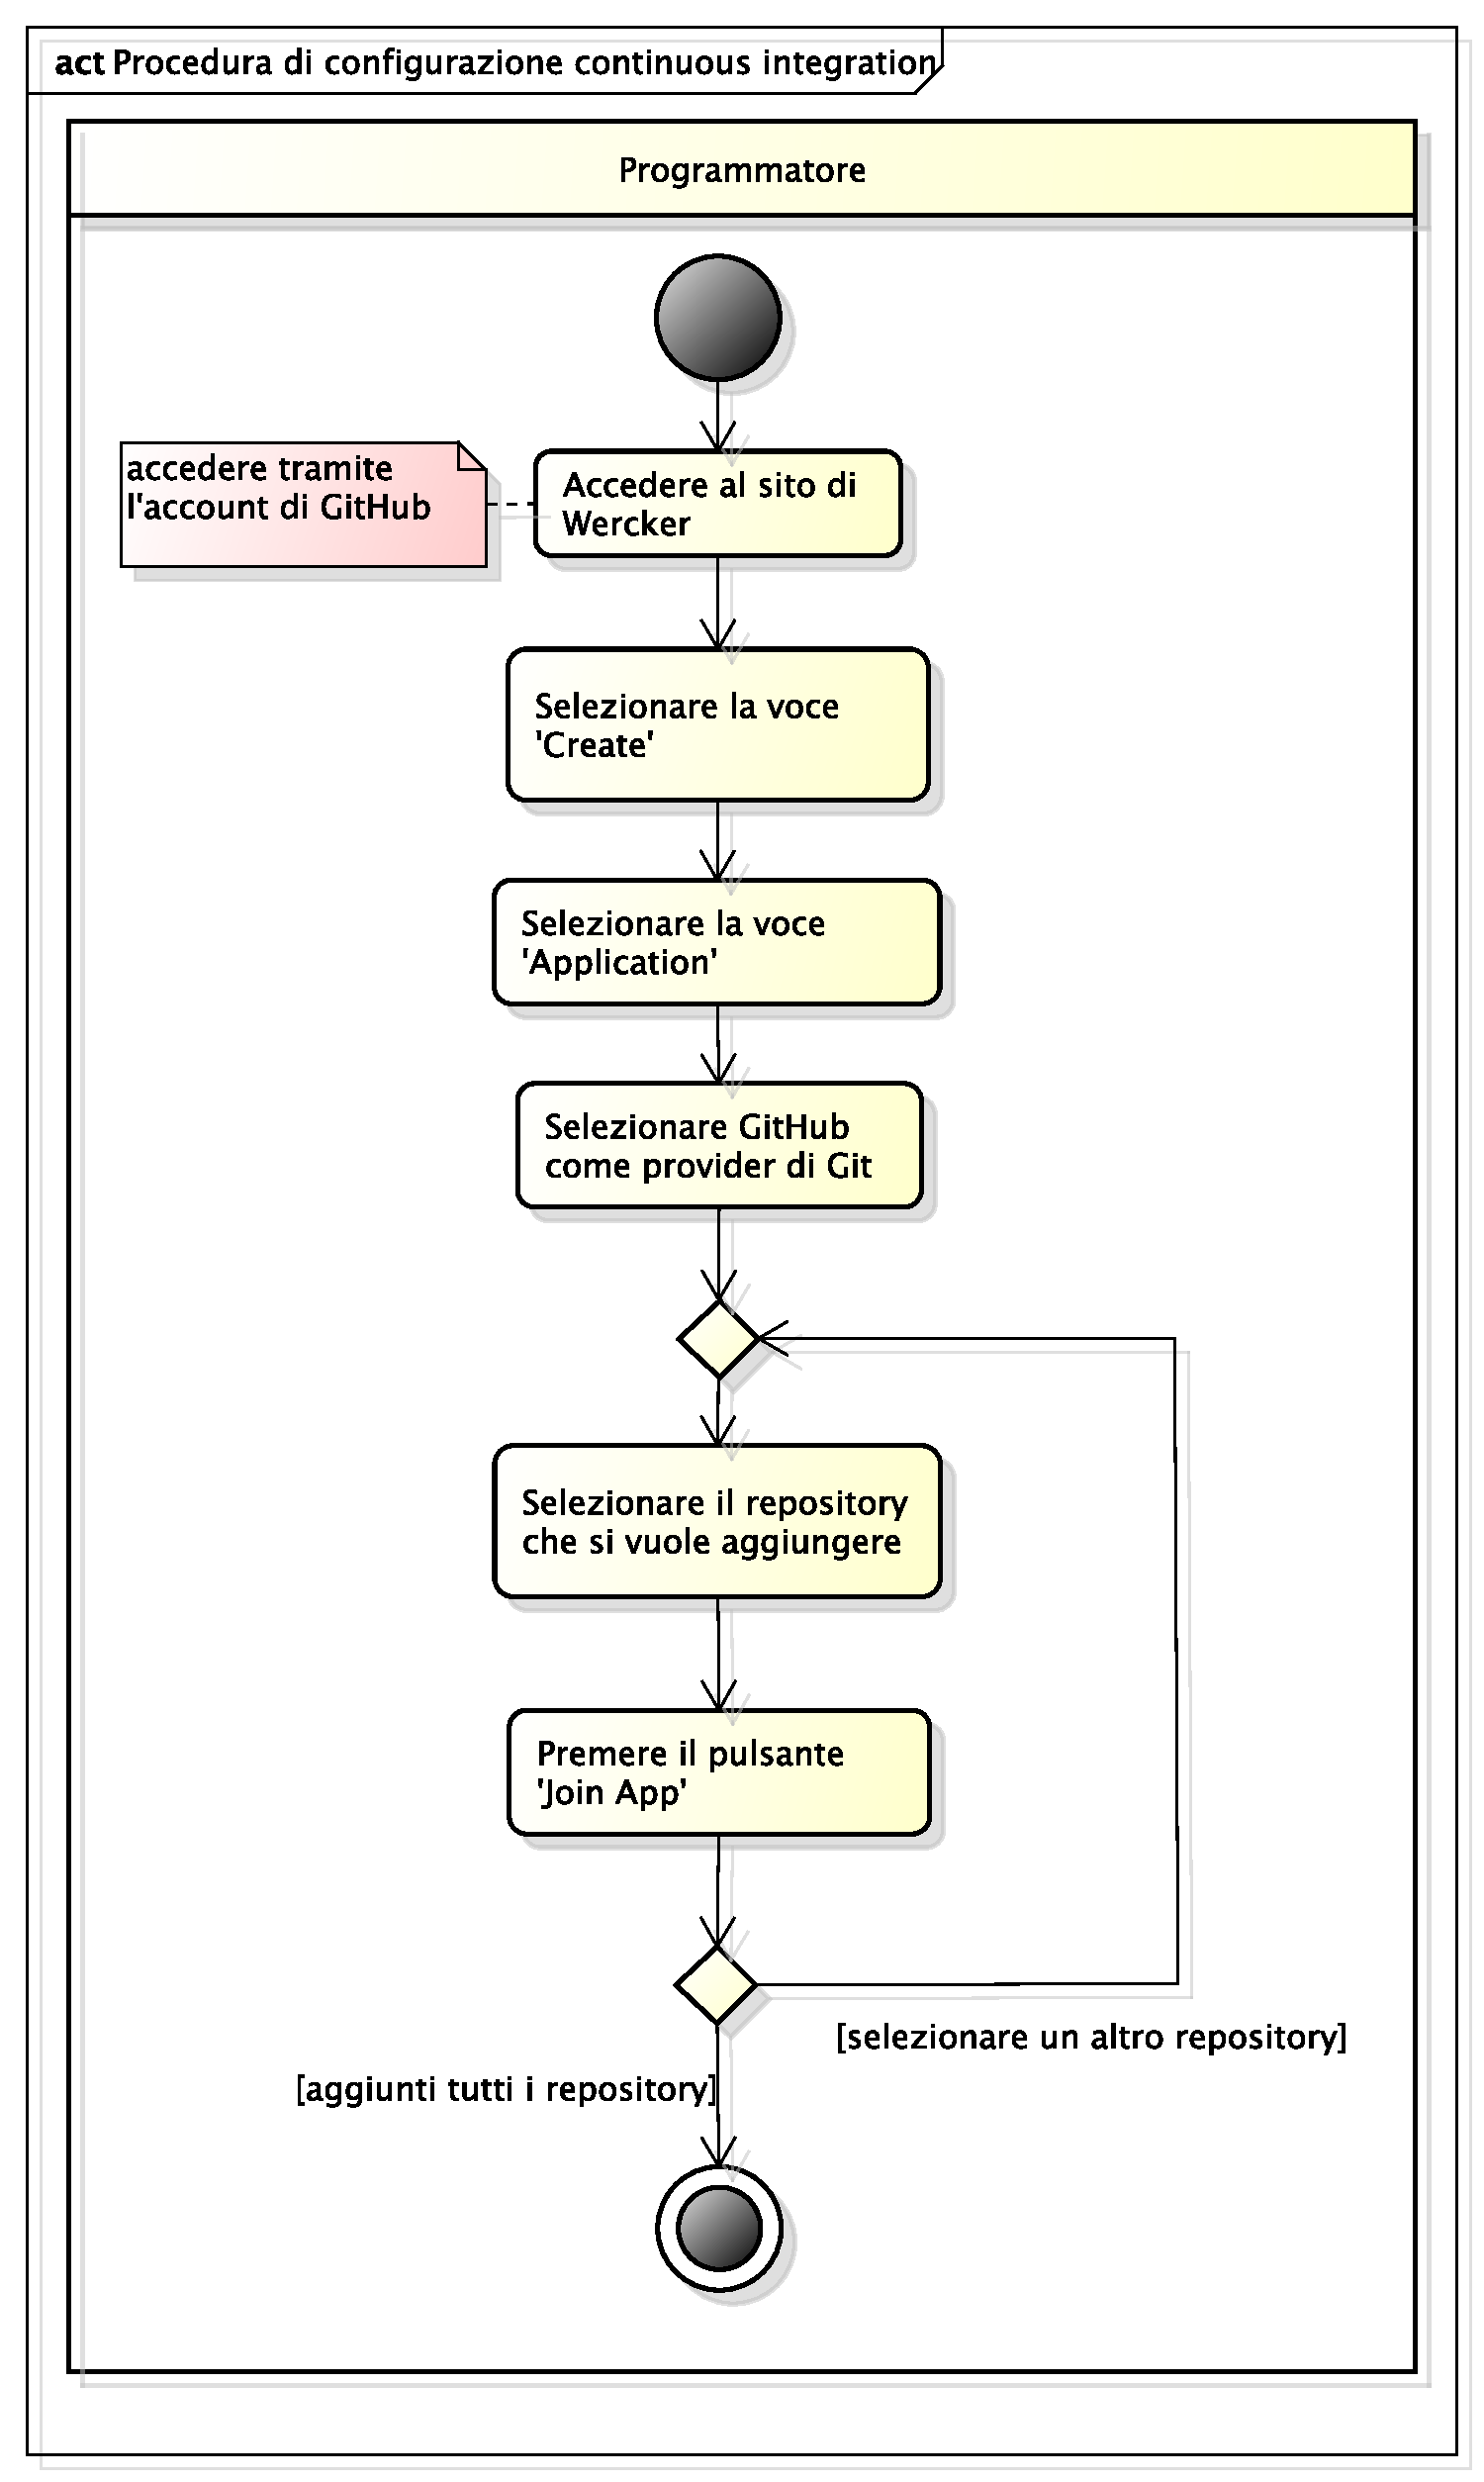
\includegraphics[scale=0.5]{images/proc_aggiunta_wercker.pdf}
					\caption{Diagramma di attività - procedura configurazione continuous integration}
					\label{fig:procedura_assegnazione_anomalie}
				\end{figure}
			% paragraph procedura_di_configurazione_sistema_di_continuos_integration (end)
		% subsubsection procedure (end)


		\subsubsection{Norme}
		\label{ssub:norme}

			\paragraph{Priorità risoluzione anomalie}
			\label{par:priorita_risoluzione_anomalie}
			Ogni anomalia riportata nel sistema deve avere una priorità di esecuzione. Di seguito vengono definite le possibili scelte:
			\begin{itemize}
				\item \textbf{P0}: priorità elevata, la risoluzione deve avvenire entro le 24 ore dalla notifica;
				\item \textbf{P1}: priorità media, la risoluzione deve avvenire entro 3 giorni dalla notifica;
				\item \textbf{P2}: priorità normale, la risoluzione deve avvenire entro 7 giorni dalla notifica;
				\item \textbf{P3}: priorità bassa, la risoluzione deve avvenire entro 2 settimane dalla notifica;
			\end{itemize}
		% subsubsection norme (end)


		\subsubsection{Strumenti} % (fold)
		\label{ssub:verifica_strumenti}
			\paragraph{Correzione ortografica} % (fold)
			\label{par:correzione_ortografica}
			Per la parte di correzione ortografica, si sono scelti di usare due strumenti di analisi. Il primo risiede all'interno dell'editor TexMaker, offrendo le funzionalità di correttore ortografico per i file \LaTeX. Esso ha dei limiti, in quanto usa un normale dizionario presente all'interno del sistema operativo e può essere utile per gli errori più grossolani di ortografia. \\
			Per ovviare al problema, si è scelto di implementare ulteriormente un controllo più accurato tramite il software \emph{GNU Aspell}. Esso permette una migliore integrazione con i file \LaTeX{} e permette l'aggiunta centralizzata dei termini di più difficile comprensione.
			% paragraph correzione_ortografica (end)

			\paragraph{Calcolo indice Gulpease} % (fold)
			\label{par:calcolo_indice_gulpease}
			Attraverso i file di testo, generati in automatico per ogni documento dallo script elencato nella sezione \ref{par:script_doc}, l'\roleAdministrator{} potrà confrontarne la conformità con le metriche previste dal \docNameVersionPdQ.
			% paragraph calcolo_indice_gulpease (end)


			\paragraph{Cloc} % (fold)
			\label{par:cloc}
			Cloc è lo strumento che viene utilizzato per il calcolo di alcune metriche stabile del \docNameVersionPdQ{} come il conteggio delle linee di commento e quelle di codice effettivo.
			% paragraph cloc (end)

			\paragraph{Wercker} % (fold)
			\label{par:wercker}
			Wercker è lo strumento scelto per le attività di Continuous Integration. \'E disponibile come applicazione cloud, non necessitando quindi di essere scaricato in locale. Questo consente di non dover provvedere a possibili diverse configurazioni nelle macchine dei diversi membri del gruppo. Sarà compito dell'\roleAdministrator{} impostare inizialmente i settaggi necessari a far funzionare l'applicativo.
			% paragraph wercker (end)


			\paragraph{Karma} % (fold)
			\label{par:karmajs}
			Karma è uno strumento che permette di eseguire del codice JavaScript in più browser o di testarlo in diverse maniere e in diversi momenti. \newline
			Viene configurato direttamente quando si installa Yeoman attraverso il generatore di angular utilizzato.
			% paragraph karmajs (end)

			\paragraph{Jasmine} % (fold)
			\label{par:jasmine}
			Jasmine è un framework JavaScript di sviluppo basato sul comportamento che viene utilizzato per testare l'applicazione, in particolare per programmare i ``test di unità''. Fornisce delle funzioni che aiutano a strutturare i test e che permettono di fare delle asserzioni. \newline
			Viene configurato direttamente quando si installa Yeoman attraverso il generatore di angular utilizzato.
			% paragraph jasmine (end)

			\paragraph{Protractor} % (fold)
			\label{par:protractor}
			Protractor è un framework JavaScript di test ``end-to-end (e2e)'' per le applicazioni in AngularJS che permette di simulare le interazioni dell'utente. Utilizza Jasmine \ref{par:jasmine} per la sintassi dei test. Viene consigliato l'uso di questo strumento al posto del deprecato \textbf{Angular Scenario Runner}. \newline
			Non è presente di default negli strumenti impostati da Yeoman. Verrà quindi configurato dall'\roleAdministrator{} prima che gli altri componenti vadano a codificare questo tipo di test.
			% paragraph protractor (end)


			\paragraph{Python unittest}
			\texttt{unittest} è un modulo integrato in Python che fornice un framework per effettuare i test di unità di tutti i moduli Python presenti nell'applicativo. Tra le diverse cose, \texttt{unittest} fornisce una classe base su cui definire diversi test e metodi per avviare il testing dell'applicativo.
			% paragraph python_unittest (end)

			\paragraph{GAE testbed} % (fold)
			\label{par:testbed_gae}
			\texttt{testbed} è un modulo Python fornito da Google che permette di testare in locale le componenti che saranno ospitati in Google App Engine fornendo dei servizi stub, dei metodi che simulano i vari servizi offerti da Google Cloud Platform.  In quanto tale modulo necessita che l'SDK di Google App Engine sia presente nel path di sistema, sarà compito dell'\roleAdministrator{} configurarne l'utilizzo in modo tale che rimanga uniforme per tutte le macchine che lo utilizzeranno.
			% paragraph testbed_gae (end)

		% subsubsection strumenti (end)
